\chapter{Theoretical Background}

\section{Time Series Analysis}

Traditional time series analysis is concerned with finding statistical information of observations distributed in time. The purpose can be to get a better understanding of the underlying process, or to make predictions on future realisations of the process. Such processes are typically present in the fields of finance, signal processing, weather forecasting, control engineering etc. Several methods for modelling processes have been developed, where some of the oldest and most useful methods are the \textit{autoregressive} model (AR) and the \textit{moving average} model (MA). These two concepts can be combined to benefit from both models into an ARMA-model.

\subsection{Autoregressive (AR) Model} \label{sub:ar}
An auto-regressive model of order $p$ is simply a linear combination of the $p$ previous terms plus some noise. An AR(p)-process is commonly characterized by its generating polynomial $A(z) = a_0 + a_1z + \cdots + a_pz^p$, where $a_i \in \mathbb{R} \ \forall \ i$ and $a_0=1$. Furthermore, let $e_t$ be uncorrelated white noise with variance $\sigma^2$ in discrete time defined as, 
\begin{align}
    \text{E}[e_t] &= 0 \label{eq:wne}\\
    C[e_s, e_t] &= \begin{cases}
    \sigma^2 \ \text{if} \ s=t \\
    0 \ \text{else}
    \end{cases} \label{eq:wnc}
\end{align}

Supposing $A(z)$ is a stable polynomial of degree $p$ and $e_t$ is as defined above, the stationary sequence $X_t$ is called an AR(p)-process with generating polynomial $A(z)$. 
\begin{align}
    X_t + a_1 X_{t-1} + \cdots + a_p X_{t-p} = e_t
    \label{eq:ar}
\end{align}

The process is stable if the roots of the characteristic equation $z^p A(z^{-1}) = 0$ are all inside the unit circle. The values $e_t$ are the called the innovations to the process and the coefficients of the $A(z)$-polynomial are tuneable parameters \citep{lindgren2014stationary}. 

There are several techniques for estimating the coefficients of the $A(z)$-polynomial. One technique is to transform the problem onto regression form and view the $A(z)$-coefficients as regression coefficients. The most recent value $X_t$ is set as the response variable $y_t$ and the previous samples $(-X_{t-1},\dots,-X_{t-p})$ are the explanatory variables $\mathbf{x}_t$. Letting the coefficients $(a_0, a_1,...,a_p)^T = \mathbf{A}$, Eq. \ref{eq:ar} can be rewritten on a vector form, recognized from regression. 

\begin{align}
    y_t = \mathbf{x}_t \mathbf{A} + e_t
\end{align}

The elements of $\mathbf{A}$ can then be estimated as the least squares estimate over $n$ samples, i.e. the values of $\mathbf{A}$ that minimize \ref{eq:leastsq}. 

\begin{align}
    L(\mathbf{A}) = \sum_{t=p+1}^n (y_t - \mathbf{x_t} \mathbf{A})^2 \label{eq:leastsq}
\end{align}

Or more conveniently, in matrix format. 

\begin{align}
    \mathbf{Y} = \begin{pmatrix}
    y_{p+1} \\
    y_{p+2} \\
    \vdots \\
    y_n
    \end{pmatrix} , \hspace{1em} \mathbf{E} = \begin{pmatrix}
    e_{p+1} \\
    e_{p+2} \\
    \vdots \\
    e_t
    \end{pmatrix} , \hspace{1em} \mathbf{X} = \begin{pmatrix}
    \mathbf{x}_{p+1} \\
    \mathbf{x}_{p+2} \\
    \vdots \\
    \mathbf{x}_{t}
    \end{pmatrix} \\[10pt] 
    L(\mathbf{A}) = (\mathbf{Y} - \mathbf{X}\mathbf{A})^T(\mathbf{Y} - \mathbf{X}\mathbf{A})
    \label{eq:leastsqmat}
\end{align}

Differentiating \ref{eq:leastsqmat} with respect to $\mathbf{A}$ and setting equal to zero yields the least squares estimate. 

\begin{align}
    \frac{\partial L}{\partial \mathbf{A}} &= -2 \mathbf{X}^T \mathbf{Y} + 2\mathbf{X}^T \mathbf{X} \mathbf{A} \\
    \frac{\partial L}{\partial \mathbf{A}} &= 0 \implies \hat{\mathbf{A}} = (\mathbf{X}^T \mathbf{X})^{-1} \mathbf{X}^T \mathbf{Y}
 \end{align}

The estimated innovation variance $\hat{\sigma^2}$ is simply the sample variance of the innovations.

\begin{align}
    \hat{\sigma^2} =\frac{1}{n-p} \sum_{t=p+1}^n e_t^2 = \frac{L(\hat{\mathbf{A}})}{n-p}
\end{align}

The method above yields an estimate for an AR(p)-process. The order $p$ of the process still has to be determined using appropriate goodness-of-fit criteria such as Akaike information criterion \citep{lindgren2014stationary}. 



\subsection{Moving Average (MA) Model}

Another popular time series model is the moving average (MA) model. This model is defined similarly to the AR-model by its generating polynomial, here called $C(z)$. 

\begin{align}
    C(z) = c_0 + c_1 z + \cdots + c_q z^q 
\end{align}

A MA(q)-process is a linear combination of the $q$ previous white noise terms as defined in Eqs. \ref{eq:wne} and \ref{eq:wnc}, plus one new innovation term:

\begin{align}
    X_t = e_t + c_1 e_{t-1} + \cdots + c_q e_{t-q}
\end{align}

A common adjustment to the model is to set $c_0 = 1$ and adjust the other coefficients and the innovation variance accordingly. 

An important distinction between the AR(p)-process and the MA(q)-process that the covariance function for the MA(q)-process is zero for time lags $\tau$ larger than the order q of the process. In other words, the value $X_{t+q + 1}$ is independent of the value $X_t$ in an MA(q)-process \citep{lindgren2014stationary}. 

\subsection{Autoregressive Moving Average (ARMA) Model}


The AR-process and MA-process are commonly combined into an ARMA-process. Letting the noise on the right hand side of Eq. \ref{eq:ar} be an MA(q)-process, the expression of an ARMA(p,q)-process is achieved. 

\begin{align}
    X_t + a_1 X_{t-1} + \cdots + a_pX_{t-p} = e_t + c_1 e_{t-1} + \cdots + c_q e_{t-q}
    \label{eq:arma}
\end{align}

There are various methods for estimating the coefficients of the polynomials $A(z)$ and $C(z)$. One is a regression approach similar to the method described in Sect. \ref{sub:ar}, where regression samples are constructed from the time series and the coefficients are estimated in a least squares sense. Another common estimation procedure is to use maximum likelihood estimation of the parameters. Assuming the noise follows some distribution -- most commonly Gaussian -- a distribution can be calculated for the model coefficients. The likelihood of obtaining a given set of a parameters can then be calculated and optimized \citep{hamilton1994time}. 

\section{Representation of Language}

Language has enabled people to exchange information in an efficient manner for thousands of years, both through speech and text. The complexity and nuances that makes a language so fitting for transferring information between humans is also what makes it so difficult to represent in numbers. A few of the difficulties when interpreting text language are listed below. 
\begin{description}
    \item[Homonyms.] Words that have the same spelling but different meaning. Consider for instance the word \textit{bull}, which might refer to the animal or an investor who believes in a rising market. The same letters, but with vastly different interpretations depending on the context. 
    \item[Negations.] The sentences \textit{God will help you} and \textit{No God will help you} contain almost the same words, but have completely opposite meanings. 
    \item[Sarcasm/irony.] This can be hard enough to detect for humans. The phrase \textit{That's just what I needed today!} might actually mean what it literally says, or just the opposite.
\end{description}

Methods used for representing words deal with these difficulties in different ways or not at all. For some shallow, more simple NLP tasks, a model might perform well without understanding homonyms or that two words are closely related. For more complex tasks such as sequence-to-sequence translation of language, a deeper understanding is naturally needed.

\subsection{One-hot Encoding}
The most intuitive way to turn words into numerical vectors is probably one-hot encoding. Thi is simply done by giving all unique words in a text an index and then letting the index represent the word. Consider a training example $x_i$ as the sentence below:

\begin{quote}
A gorilla visited Manilla.
\end{quote}

The first processing needed is to divide the sentence into smaller units -- \emph{tokens}. A tokenized version of the sentence above would be:
\begin{verbatim}
['A', 'gorilla', 'visited', 'Manilla', '.']
\end{verbatim}

Some of these tokens carry information about the beginning or end of the sentence, which is obviously important. However, not all capital letters imply the start of a sequence and not all punctuation indicates the end of a sequence, e.g. \textit{Hello Mr. Gorilla!}. There are quite a few special cases of this sort, and there are convenient functions in Python that deal with the problems of tokenization, such as \textit{Tokenizer} from Keras \citep{chollet2020keras}. The tokenizer from Keras splits the text into sequences, removes the punctuation and transforms all characters to lower case by default. 

When the sentence is tokenized, it is also common to remove the most frequent words, since these probably don't give a lot of information about the difference between sentences. These are called \textit{stop words} and typically include common words such as \textit{a, the, but}, etc.

After the tokenization, each unique word is given an index. 
\begin{center}
    \begin{tabular}{rc}
        \textit{gorilla} $:$ & 1 \\
        \textit{visited} $:$ & 2 \\
        \textit{manilla} $:$ & 3 \\
    \end{tabular}
\end{center}

Each word of the sentence is then transformed to a one-hot vector where all elements are zero except for element $i$. A sequence of words can then be represented as a sequence of vectors. 

\begin{align*}
    \textit{gorilla} : \begin{bmatrix}
    1 & 0 & 0 
    \end{bmatrix} \\
    \textit{visited} : \begin{bmatrix}
    0 & 1 & 0 
    \end{bmatrix} \\
    \textit{manilla} : \begin{bmatrix}
    0 & 0 & 1 
    \end{bmatrix} \\
\end{align*}


\subsection{Bag-of-words \& TF-IDF}

An initial \emph{bag-of-words} (BOW) approach to represent a sentence as a vector is to simply keep track of whether a word is included in the sentence or not. If the word is included, the element on the corresponding index has value 1, otherwise 0. Using the same indices as previously and removing stop words, \emph{A gorilla visited Manilla} would then be represented by $x_i$ as, 

\begin{align*}
    x_i = \begin{bmatrix}
    1 & 1 & 1 
    \end{bmatrix}
\end{align*}

Note that even though the order of words is the same in the vector as in the original sentence, this is not necessarily the case. The less interpretable sentence \textit{Manilla visited a gorilla} would have the same vector representation as $x_i$. Hence, BOW does not take order of words in a sentence into account. 

There are variations of BOW that have larger representing power, such as including the count of words in the sentence rather than if it exists or not. A problem with this approach is that words that are more frequent in sentences get a higher value than words that are not as frequent, even if less frequent words might be more interesting for the context. A variation that deals with this limitation is the TF-IDF representation. 

Term Frequency-Inverse Document Frequency (TF-IDF) is a widely used technique for normalizing text data. It uses the same underlying principles as BOW but with a weight normalization. As the name suggests, the value for a certain word is increased for its frequency in a document but decreased for the frequency in the full corpus. So, a word which has a low frequency in a full corpus is considered more important than a word with high frequency. The entry for a word with index $j$ in a sample vector $x_i$ is then calculated as the product of the term frequency weight and the inverse document frequency weight. 

\begin{align*}
    x_{ij} = f_s(t,f) \cdot f_d(t,F)
\end{align*}

For a term $t$ with frequency $f$ in sequence $i$ and frequency $F$ in the whole corpus. The function $f_s$ is some function increasing with the number of words $j$ in the sentence and $f_d$ is decreasing with the number of words in the full corpus. Examples of these functions can be as below. 

\begin{align*}
    f_s &= \frac{\mid \{ j \in (1, \hdots , L_i) : s_{ij} = t  \} \mid}{L_i} \\
    f_d &= \log{\frac{N}{n_t}}
\end{align*}

Where $L_i$ is the length of the sentence $i$, $N$ is the number of sequences in the document and $n_t$ is the number of documents in which the term $t$ occurs at least once \citep{manning2008introduction}.

While this remedies some of the shortcomings of BOW, there are still some aspects where it falls short: 
\begin{enumerate}
    \item Firstly, the size of the vectors grows with the number of unique words in the corpus, which becomes computationally infeasible for larger texts. 
    \item Secondly, the order of the words is not accounted for in BOW. When used in an application for interpreting financial news, the representation must be able to distinguish between \textit{Google placed a bid on Amazon} and \textit{Amazon placed a bid on Google}. BOW however simply registers the occurrence of words. 
    \item Finally, BOW does not really capture any essence of the language. There is no way for the mode to capture the similarity between words such as \textit{awesome} and \textit{amazing}. This is related to the large dimensionality of the vectors representing the words, since each word has a unique dimension in the vector. This implies all dimensions are orthogonal, therefore there is no usable algebraic measure of similarity. 
\end{enumerate}

All of the problems above are addressed by the concept of word embeddings in the next section. 

\subsection{Word Embeddings}
As opposed to the sparse representation of one-hot encoding, \textit{word embeddings} are dense, continuous vector representations of words. The dimension of a one-hot encoded vector corresponds to the size of the vocabulary (generally 20,000 or greater), whereas word embedding vectors typically have 100 to 1000 dimensions \citep{chollet2017deep}.

A major breakthrough on the topic of word embeddings was made by \citet{mikolov2013efficient}, where efficient methods of training a model were introduced, popularised as the \textit{word2vec} model. \textit{Continuous bag-of-words} and \textit{continuous skip-gram} are two model architectures for training the $d$-dimensional vector representations of words. Both methods share the notion that the meaning of a word is determined by the words it is commonly used together with. The representations are learned by constructing a language modeling task which is solved by a neural network. The task is generally to predict neighboring words of a given word. The weights into the hidden layer of the trained neural network are the embeddings for a word. 

\textit{Continuous bag-of-words} are trained by predicting the missing word in a sequence of words of a given window size. The order of the words is not taken into consideration other than for deciding which words to include in one sequence. For instance, the phrase \textit{A gorilla visited Manilla} with window size one gives the following training samples.
\begin{center}
\textit{A gorilla visited} $\implies x = $ \textit{(a, visited)} $,y = $ \textit{gorilla} \\ \vspace{1em}
\textit{gorilla visited Manilla} $\implies x = $ \textit{(gorilla, Manilla)} $,y = $ \textit{visited} \\
\end{center}


\textit{Continuous skip-grams} also use the fact that words that often occur together have some sense of similarity, but is in a way the inverse of continuous bag-of-words. Rather than predicting the missing word, the objective of the model is to predict the surrounding words. To construct training examples from the same phrase as above with a 1-skip-gram, the following samples are generated. 

\begin{center}
\textit{A gorilla visited} $\implies x, y_1, y_2 = $ \textit{gorilla, a, visited} \\ \vspace{1em}
\textit{gorilla visited Manilla} $\implies x,y_1, y_2 = $ \textit{visited, gorilla, Manilla}
\end{center}

The known words above are \textit{gorilla} and \textit{visited} respectively.

According to the authors\footnote{See for instance: \url{https://code.google.com/archive/p/word2vec/}}, the continuous bag-of-words model is faster for training but the continuous skip-gram model is better for infrequent words. 

The word embeddings generated by these methods do carry some information about the semantic relationship of words. As mentioned in the previous section, a desirable function of word representation is to determine whether a word is close to another word in a semantic meaning. This is elegantly represented in word embeddings as the cosine similarity between word vectors. Consider for instance the word \textit{Sweden}. The closest word vectors in the word2vec-vocabulary with respect to cosine similarity are displayed in Table~\ref{tab:cossim}.

\begin{table}[h!]
    \centering
    \begin{tabular}{lr}
    \hline
        \textbf{Word} & \textbf{Cosine similarity}  \\
        \hline \hline 
        Finland & 0.8085 \\
        Norway  & 0.7706 \\
        Denmark & 0.7674 \\
        Swedish & 0.7404 \\ 
        Swedes  & 0.7133 \\
        \hline 
    \end{tabular}
    \caption{Word vectors with the highest cosine similarity to \emph{Sweden}. Pre-trained embeddings from the word2vec module of the python gensim library were used.}
\label{tab:cossim}
\end{table}

There is also a straight forward interpretation of elementwise addition and subtraction of these word embeddings. In some sense, the $d$-dimensions of the embeddings can be interpreted to be metrics of different properties. For instance, the sum of the embeddings for the words \emph{doctor} and \emph{animal} is most similar to the embedding for the word \textit{veterinarian}. There is also reasonable syntactic results when performing simple mathematical operations. It would for instance be expected that the difference between \emph{running} and \emph{run} is similar to the difference between \emph{swimming} and \emph{swim}. This can roughly be expressed as below. 
\begin{align}
    \emph{running - run} \approx  \emph{swimming - swim}
\end{align}

Indeed, taking the embeddings for the words and calculating \emph{running - run + swim} results in a vector which is most similar to the embedding for the word \emph{swimming} using the 44,000 most common words in the python gensim implementation of word2vec.


\section{Classification Models}

The text vectorization methods presented in the previous section extracts features from raw text to a vector. This is then used as input to more general classification models which are not exclusive for natural language processing. These models are briefly covered in Section \ref{sec:treeff}. 

In other models, the text is entered as a sequence. One way to handle this is using recurrent models, which take the order of words into account. These models are covered in Section \ref{sec:recmods}. 

A recent addition to the family of NLP-models are transformer based models, where the concept of attention between words are central. Transformer models are the subject of Section \ref{sec:trfmod}.

\subsection{Tree-based \& Feed Forward Models}\label{sec:treeff} 

\paragraph{Random Forests.}
A random forest classifier is an ensembling technique, consisting of several decision trees. Predictions are made by taking the mode (for classification) or the average (for regression) of the predictions from all of the decision trees. Each decision tree in a random forest classifier is fitted to a bootstrap sample of the training set. Every tree is likely to overfit to the data it is presented with, but the full forest of trees has better generalizability as a consequence. The random forest model is a widely popular model which tends to work well without much tuning out of the box for shallow machine learning tasks \citep{chollet2017deep}. 

\paragraph{Logistic Regression.}

Logistic regression is a commonly used baseline for machine learning classification tasks. Even though it is an old model, it can still provide good results for a wide range of classification tasks \citep{chollet2017deep}. 

\paragraph{Support Vector Machines.}

Support vector machines are a group of models which can be used for both classification and regression. The core idea of a classification support vector machine is to find a suitable decision boundary between data points of different classes. This decision boundary is a hyper plane in some dimension depending on the number of features in the input data. The input data is mapped to a higher dimensional representation where the samples are easier to separate. This is however only efficient if a \emph{kernel function} can be constructed, i.e. a mapping $k$ which satisfies $k(x,y) = \varphi(x) \cdot \varphi(y)$ for some function $\varphi$. The best decision boundary is then found by maximizing the distance between the closest samples and the hyper plane in the high dimensional representation. Support vector machines can quickly make predictions on unseen data since the new sample only has to be evaluated against the decision boundary consisting of the hyper plane in the high dimensional representation \citep{chollet2017deep}.   

\paragraph{Multi Layer Perceptron.}
A multi layer perceptron, or feed forward network, is a neural network that seeks to approximate some function $f$. For a classifier, this function would map features $x$ to some prediction $\hat{y}$ of the true value $y$. The prediction depends on the weights and biases $w,b$ of the network.  

\begin{figure}[t]
    \centering
    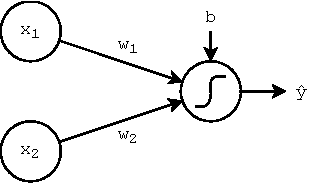
\includegraphics[width=0.4\textwidth]{Figures/figs-perceptron.pdf}
    \caption{A single perceptron unit with two inputs $x_1, x_2$, two weights $w_1, w_2$ and one bias $b$. The sigmoid in the prediction node is an activation function usually denoted $\sigma(x)$.}
    \label{fig:perceptron}
\end{figure}

The core part of the multilayer perceptron is the single perceptron unit displayed in Figure~\ref{fig:perceptron}. It is easy to see that the prediction $\hat{y}$ is a function of the inputs, weights and biases as $\hat{y} = \sigma(x_1 w_1 + x_2 w_2 + b)$, where $\sigma$ is the activation function denoted by a sigmoid in the figure. 

The training of the model will select the weight and biases such that the predictions are as accurate as possible. The bias term $b$ is usually included in the term \textit{weights} as $w_0$. This is made possible by adding an extra feature $x_0 = 1$, implying $b = w_0 x_0 = w_0$. This simplifies notation, especially for matrices. 

The performance of classification is measured by some loss function $J$, which depends on the training samples $(x,y)$ and the weights $w$.  A common loss function for binary classification is binary crossentropy, defined in Eq. \ref{eq:bce}. The notation is such that $y$ is the true label, $\hat{y}$ is the predicted label and $p(\hat{y})$ is the predicted probability of the sample being of label 1. Conversely, $1 - p(\hat{y})$ is the probability of the sample being of label 0. 

\begin{align}
    L(y,\hat{y}) = -\frac{1}{N} \sum_{i=1}^N y_i \log{(p(\hat{y}_i))} + (1 - y_i) \log{(1 - p(\hat{y}_i))} \label{eq:bce}
\end{align}

A single perceptron unit is not too exciting, but when combined into a network, it is more powerful. \citet{leshno1993multilayer} proved that a neural network with a locally bounded piecewise continuous activation function can approximate any continuous function to any degree of accuracy if and only if the activation function is not a polynomial. This is known as the universal approximation theorem. While this implies that a sufficiently large multi layer perceptron is able to represent any continuous function, it does not guarantee that a network is able to learn this representation. Furthermore, the size of the network is unrestricted and can in practice be infeasible computationally \citep{Goodfellow-et-al-2016}. 


\begin{figure}[t]
    \centering
    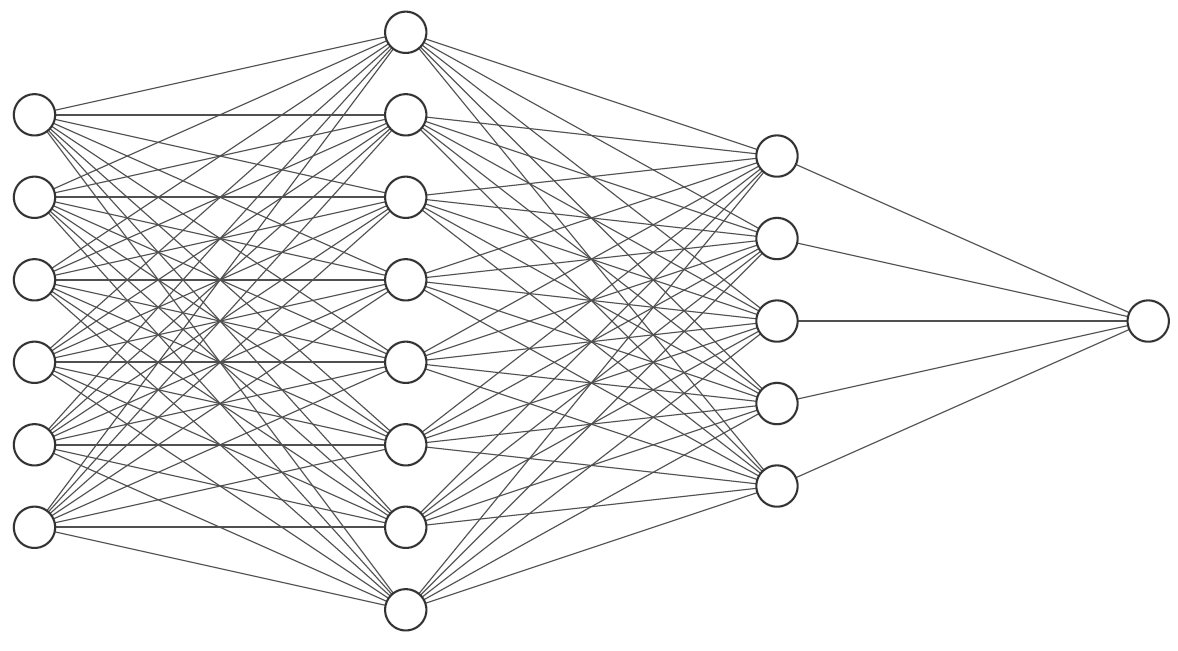
\includegraphics[width=0.7\textwidth]{Figures/ff.PNG}
    \caption{Overview of a densely connected feed forward network with six inputs, two hidden layers and one output node.}
    \label{fig:mlp}
\end{figure}

Combining the basic functionality in Figure~\ref{fig:perceptron} with the network in Figure~\ref{fig:mlp}, a neural network is achieved. This can function as both a regression and classification model. For regression, the activation function in the final node is typically a linear function as $\varphi(x) = cx$, for some real constant $c$. For classification, it is usually some sigmoid function bounded between 0 and 1, such as $\displaystyle{\varphi(x) = \frac{1}{1 + e^{-x}}}$. The most popular activation function in the nodes which are inside the network is the rectified linear unit function (ReLU), defined as $\varphi(x) = \max(0,x)$ \citep{Goodfellow-et-al-2016}. These functions are all conveniently implemented in Keras, as well as a structure using different layers to build a model \citep{chollet2020keras}. 

\subsection{Recurrent Models}\label{sec:recmods}

A drawback which affects all of the models presented in the previous section is that the order of words is not taken into account. Of course, the order can be considered in the pre-processing if some more complex transformation is used (e.g. Sentence-BERT), but these transformations usually utilize some recurrent or attention-based method. A recurrent model takes the sequence order into account. 

\paragraph{Recurrent Neural Networks.}

A recurrent neural network (RNN) is rather similar to a multilayer perceptron, but it takes previous inputs into account. The input to an RNN is a sequence of samples. In natural language processing, a sequence is typically a sentence. An RNN can however be used for other tasks where the order of samples are important, e.g. time series forecasting.

Obviously, a sentence can not be defined just by the word it contains, one must also take the order of the words in the sentence into account. We keep a general idea of the meaning of what we have previously read and adjust the idea depending on the new words in the sentence. Recurrent neural networks work in a rather similar way, storing hidden representations of inputs and conveying that information to the next input in the sequence \citep{Goodfellow-et-al-2016}. 

\begin{figure}[t]
    \centering
    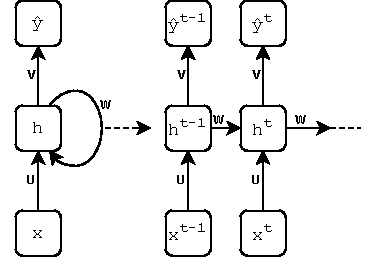
\includegraphics[width=0.5\textwidth]{Figures/figs-simplernn.pdf}
    \caption{General graph of a sequence-to-sequence RNN unfolded through time, where a sequence of inputs $x$ predicts a sequence of outputs $y$. $\mathbf{U}$, $\mathbf{V}$ and $\mathbf{W}$ are weights that are shared throughout the sequence, independent of the position.}
    \label{fig:rnn}
\end{figure}

As seen in Figure~\ref{fig:rnn}, an RNN can be seen as a feed-forward neural network where previous time steps are used as input. Assuming a hidden layer activation function $\sigma_h$ and an output activation function $\sigma_o$, the recurrent nature of the model can be further explained. Let the other notation be as in Figure~\ref{fig:rnn}. 

\begin{align}
    \hat{y_t} &= \sigma_o(V \cdot h^{(t)}) = \sigma_o(V \cdot  \sigma_h(U x^{(t)} + W h^{(t-1)})) \\
    h^{(t-1)} &= \sigma_h(Ux^{(t-1)} + W h^{(t-2)})
\end{align}
Clearly, the prediction $\hat{y}^{(t)}$ is dependent on the previous inputs $x^{(i)}$ and hidden states $h^{(i)}$. 

The model structure is similar for sequence-to-one classifications, i.e. a sequence
\[
(x_i^{(1)}, x_i^{(2)}, ..., x_i^{(l)})
\]
predicts one label $\hat{y}_i$. Given a sequence length $l$, only the final step $x_i^{(l)}$ provides an output $y_i$. This output is however influenced by the previous inputs $x_i^{(t)}$ through the hidden layers $h^{(t)}$ and the weights $W$, see Figure~\ref{fig:rnns2o}. 


\begin{figure}[t]
    \centering
    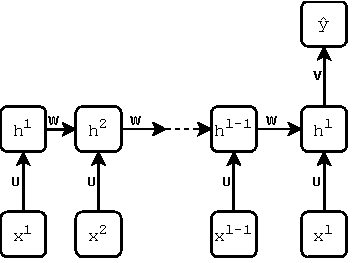
\includegraphics[width=0.5\textwidth]{Figures/figs-rnn-s2o.pdf}
    \caption{Schematic graph of a sequence-to-one RNN unfolded through time, where a sequence of inputs $(x^{(1)}, ..., x^{(l)})$ predicts one output $y$.}
    \label{fig:rnns2o}
\end{figure}

\paragraph{Long Short-Term Memory (LSTM).}
Even though the general idea of the previously described method is widely used, the model is not used precisely as described. The simple RNN-structure suffers from the \textit{vanishing gradient problem}. To understand this problem, one must understand how the network is trained, which is outside the scope of this report. In short, long term dependencies are too many time-steps away to have an impact when the network is trained. 

In practice, either Long-Short-Term Memory (LSTM) or Gated Recurrent Unit (GRU) are used instead. The main difference is that information that is deemed important is allowed to pass on to later time-steps without too much interference from hidden several dot products and activation functions. This alleviates the vanishing gradient problem, even though the core idea is the same as the previously described simple RNN \citep{chollet2017deep}.

\paragraph{Bidirectional LSTM.}
As a final note for the recurrent neural network approach, it should be mentioned that when RNNs are used in natural language processing, they are often wrapped with a bidirectional layer. This simply reverts the input sequence and enters the sequence in both the original and the reverse direction to two separate RNNs, usually LSTM or GRU. 

The usefulness of this is particularly intuitive when looking at the network in Figure~\ref{fig:rnn}. When processing the entry $x^{(j)}$, only the entries $t < j$ are known. However, tokens later in the sequence might have an impact on the previous outputs of the model. Bidirectional LSTMs can catch patterns that are overlooked by regular LSTMs.

Bidirectional LSTMs have been widely popular in the field of natural language processing. In 2017, the model behind Google Translate was powered by seven stacked LSTM layers \citep{chollet2017deep}. 

\subsection{Transformers}\label{sec:trfmod}
In \citeyear{NIPS2017_7181}, \citeauthor{NIPS2017_7181} wrote a paper, \textit{Attention is all you need}, which had a considerable influence on language modelling and machine translation. The authors presented a new model -- the Transformer -- which does away with the recurrence and instead only uses the concept of attention. One of the problems with recurrent networks is the lack of parallelizability when training the network. The Transformer allows for more parallelization than previous models and consequently trains quicker than models based on recurrence. This is proved by a new state of the art score of 28.4 BLEU on the WMT 2014 English-to-German translation task which was trained at a fraction of the training cost compared to the previous state of the art models. 


In the rest of the section, I will follow \citet{NIPS2017_7181}, as well as a more detailed description by \citet{jayalammar2018} to describe the principles behind the Transformer. The explained model is used for sequence-to-sequence modelling such as translation, but is also the foundation for BERT which can be used for classification, and is presented later. This is the motivation for this rather detailed section on transformers, even though the model itself is not used in this project. 

\begin{figure}[ht]
    \centering
    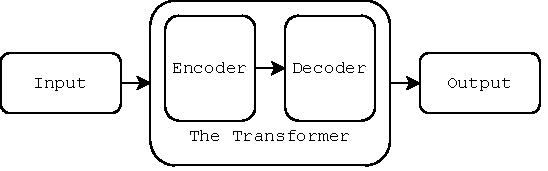
\includegraphics[width=0.5\textwidth]{Figures/figs-transformer.pdf}
    \caption{Schematic graph of a transformer.}
    \label{fig:trfo}
\end{figure}

The core idea is to encode the input into a manageable, general representation and then decode this representation into the sought output. Both the encoder and decoder parts consist of 6 identical layers of encoders and decoders.

\begin{figure}[ht]
    \centering
    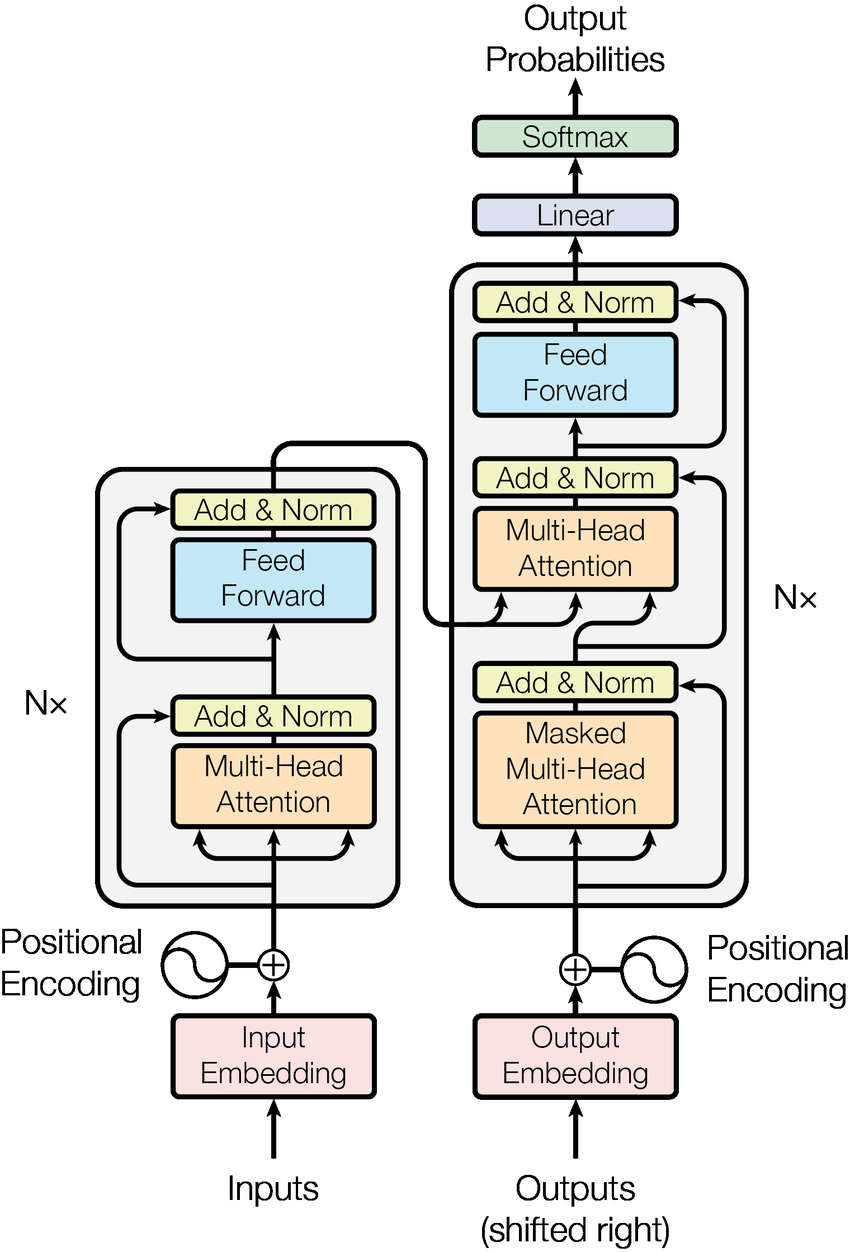
\includegraphics[width=0.5\textwidth]{Figures/The-Transformer-model-architecture.png}
    \caption{Model architecture of the transformer with the encoder to the left and the decoder to the right. The paper uses $N = 6$ layers for both the encoder and the decoder. After \citet{NIPS2017_7181}.}
    \label{fig:tr_arch}
\end{figure}

\subsubsection{Transformer Tokenization}\label{sec:transtok}

Firstly, the input to the model is tokenized in a different way than what has been described for previous models. It is similar in the sense that each token is transformed into an embedding. \citet{NIPS2017_7181} uses a WordPiece embeddings of dimension $d_{model} = 512$. The way the model handles positional information of words is however quite different. 

Rather than letting a sequential input to the model represent the position of tokens similar to an RNN, the positional information is included in sine and cosine functions with different frequencies. 

\begin{align}
    PE(pos,i) = \begin{cases}
    \sin\displaystyle{\Big(\frac{pos}{10000^{2i/d_{model}}}\Big)} \ , & i = 2k \\
    \\
    \cos\displaystyle{\Big(\frac{pos}{10000^{2i/d_{model}}}\Big) }\ , & i = 2k + 1 
    \end{cases} \   k \in \mathbb{N}
    \label{eq:posid}
\end{align}

In Eq. \ref{eq:posid}, $pos$ is the position of the token in the sentence and $i$ the dimension of the embedding. One word has one position $pos$ and $d_{model} = 512$ dimensions.

This way of representing the positions of a word might seem cumbersome at first, but it has some nice features: 

\begin{description}
    \item[Dimensional consistency.] These positional embeddings can be chosen to have the same dimension as the vectors used for the word embedding. In the original papers, the positional encodings are simply added to each element $i$ of the $d_{model} = 512$ dimensions. 
    \item[Generalizable.] This method can extrapolate to sentence lengths not seen in the training data. 
    \item[Simple relative positioning.] The fact that $PE(pos, i)$ can be written as a linear function of $PE(pos, i + k)$ for any $k$, should according to \citet{NIPS2017_7181} make it easier for the model to acknowledge relative positions. 
    \item[No recurrence.] This is not unique for this sinusoidal version of positional encoding, but is however one of the main features of the transformer, allowing for more parallel computations. 
\end{description}

\subsubsection{Encoder \& Self-Attention}

After the input embedding and positional encoding, a sample is passed through to the stack of encoder layers, shown to the left in Figure~\ref{fig:tr_arch}. This is where the concept of self-attention comes in. 

At a conceptual level, self-attention for words could be described as how much other words in the sentence represent the current word, i.e. what other words in the sentence the word pays attention to. As an example, consider the following two sentences. 

\begin{quote}
The gorilla didn't like Manilla, it was too crowded.\\
The gorilla didn't like Manilla, it was too tired.
\end{quote}

In order to interpret the sentence correctly, a model must understand that \emph{it} refers to \emph{Manilla} in the first sentence and to \emph{the gorilla} in the second. This is the purpose of the self-attention, to detect which words in the neighborhood that are important for the meaning of the current word. I explain the mathematics behind it below. 
As seen in Figure~\ref{fig:tr_arch}, there are 6 layers of multi-head attention with following feed forward layers. One multi-head attention is made up of 8 identical parallel self-attention layers. Each attention layer has unique weights. In the first layer, the inputs are simply word embeddings and positional encodings. Consider the sentence \textit{The gorilla visited Manilla} with some word embeddings $x$ and positional encodings $PE$:
\begin{quote}
\begin{tabular}{cccc}
A &gorilla &visited &Manilla\\
$x_1$&$x_2$&$x_3$&$x_4$\\
$PE_1$&$PE_2$&$PE_3$&$PE_4$\\
\end{tabular}
\end{quote}

The vector which is given to the self-attention layer is then $h^o$ as in Eq. \ref{eq:attinp}. Note that the dimension for $x, PE$ and $h^o$ is $l \times d_{model}$, where $l = 4$ in this example and $d_{model} = 512$ in the original paper. 

\begin{align}
    x &= \begin{bmatrix} x_1 & x_2 & x_3 & x_4 \end{bmatrix}^\intercal \\
    PE &= \begin{bmatrix} PE_1 & PE_2 & PE_3 & PE_4
    \end{bmatrix}^\intercal \\
    h^o &= \begin{bmatrix} x_1 + PE_1 & x_2 + PE_2 & x_3 + PE_3 & x_4 + PE_4 \end{bmatrix}^\intercal \label{eq:attinp}
\end{align}

The first calculations in the attention layer are three linear transformations to construct three vectors: a query vector, a key vector and a value vector. The matrices $W_Q, W_K$ and $W_V$ are weights which are tuned during the training and determine the query, key and value vectors. 

\begin{align}
    q_i = h_i^o W_q \\
    k_i = h_i^o W_k \\
    v_i = h_i^o W_v 
\end{align}

These vectors are used to calculate an attention score for a given word $i$ versus all other words $j$ in the sentence. The score is calculated as the dot product of $q_i$ and $k_j$ and scaled by $\displaystyle{\frac{1}{\sqrt{d_k}}}$ where the original paper uses a dimension of $d_k=64$ for the query, key and value vectors.

\begin{align}
    \text{score}_{i,j} = \frac{q_i \boldsymbol{\cdot} k_j}{\sqrt{d_k}}
\end{align}

The scaling by $\sqrt{d_k}$ is made to keep the gradients of the attention layer at a more manageable level. The scores for the word $i$ against all other words $j$ are then normalized with a softmax function, ensuring the sum over all words $j$ sums up to one and that larger scores are boosted. The softmaxed score for word $i$ against word $j$ is then calculated as in Eq. \ref{eq:softmax}.

\begin{align}
    \text{softscore}_{i,j} = \frac{e^{\text{score}_{i,j}}}{\sum\limits_{\forall j} e^{\text{score}_{i,j}}}
    \label{eq:softmax}
\end{align}

Finally, the contribution to the attention for each word is calculated by adding up all the value vectors $v_j$ weighted by the softmaxed score of $i$ and $j$. This concludes the calculation of the new hidden state $h_i^{o+1}$ for word $i$. 

\begin{align}
    h_i^{o+1} = \sum\limits_{\forall j} v_j \cdot  \text{softscore}_{i,j} 
\end{align}

 Figure~\ref{fig:attflow} shows a flow graph over how this is calculated. 

\begin{figure}[ht]
    \centering
    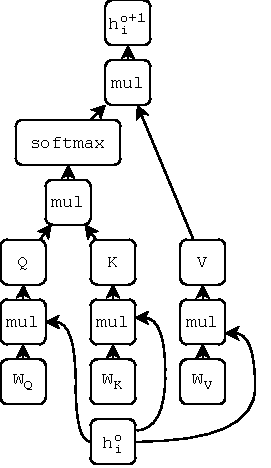
\includegraphics[width=0.4\textwidth]{Figures/figs-self-att.pdf}
    \caption{Calculation of self-attention from hidden layer $o$ to $o+1$ for word $i$. \texttt{mul} denotes a matrix multiplication or a dot product.}
    \label{fig:attflow}
\end{figure}

The details of the calculation until now have concerned one word at the time in the sentence. It can however be neatly compressed into matrix form.

Letting $h^o$ be as defined in Eq. \ref{eq:attinp}, we can  write the query, key, and value vectors as matrices where every row corresponds to the vector for a word in the sentence. 

\begin{align}
    Q = h^o W^Q \\
    K = h^o W^K \\
    V = h^o W^V
\end{align}

The attention of the layer can then be calculated as in Eq. \ref{eq:attout}, by the steps shown for one word in the previous segments. 

\begin{align}
    \text{Attention}(Q,K,V) = \text{softmax}\Big( \frac{Q K^\intercal}{\sqrt{d_k}}\Big) V
    \label{eq:attout}
\end{align}

What has been demonstrated until now is the flow for a sample through one attention layer. However, the transformer model uses a multi-head attention layer. This is simply 8 attention layers that run in parallel. The weights across the layers are not shared, but the idea is that having eight attention layers with random initialization enables focusing on different aspects of language. The output of the eight layers are concatenated and multiplied by another matrix of weights $W^O$ in order to reduce the dimensions to $l \times d_{model}$, which are the same dimensions as was fed to the model in Eq. \ref{eq:attinp}. 

Note that the first inputs to the model are word embeddings and positional encodings, but the rest of the encoder layers has the output from the previous layer as input, which is of the same dimension as the input embeddings. 

The final step in the encoder layer is a position-wise feed forward network, roughly as in Figure~\ref{fig:mlp}. The network has one hidden layer of size $d_{ff} = 2048$. The input and output are both of size $d_{model} = 512$. The difference with a regular multi layer perceptron is that the weights are applied identically to each position, greatly reducing the number of tuneable weights. The hidden layer has ReLU activation functions, so the output for any input can be conveniently written as in Eq. \ref{eq:attmlp}

\begin{align}
    F(x) = \max(0, x W_1 + b_1)W_2 + b_2)\label{eq:attmlp}
\end{align}

Another important property of the Transformer is the residual connections seen in Figure~\ref{fig:tr_arch}. These allow information to be transferred to a new layer without being distorted in the attention calculations. \citet{NIPS2017_7181} claim this is particularly important for the positional encodings to stay intact deeper into the network. 

\begin{figure}[h]
    \centering
    \begin{minipage}{\textwidth}
        \centering
        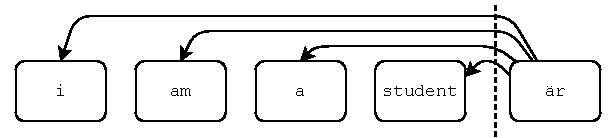
\includegraphics[width=0.6\linewidth]{Figures/figs-enc-dec-att.pdf}\par
        \emph{Encoder-decoder attention}
    \end{minipage}\vspace{1em}
    \begin{minipage}{0.49\textwidth}
        \centering
        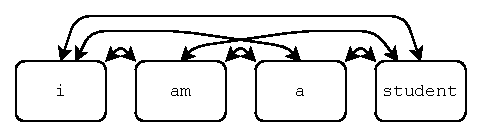
\includegraphics[width=\linewidth]{Figures/figs-enc-self-att.pdf}\par
        \emph{Encoder self-attention}
    \end{minipage}
    \begin{minipage}{0.49\textwidth}
        \centering
        \vspace{4px}
        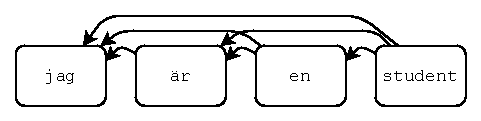
\includegraphics[width=\linewidth]{Figures/figs-dec-self-att.pdf}\par
        \emph{Decoder self-attention}
    \end{minipage}\vspace{1em}
    \caption{Different types of attention in a transformer. Imaged by a translation task from the English sentence "i am a student" to the Swedish sentence "jag är en student". }
    \label{fig:selfatts}
\end{figure}

\subsubsection{Decoder \& Output}

There are many similarities between the encoder and decoder, but some things differ. The output from the encoder is used to calculate the attention vectors $K$ and $V$ which are used to predict a sequential output from the decoder. The first input to the decoder are these attention vectors and a start-of-sequence token. These then progress through the decoder layers and produce an output. The output is made by a linear transformation to a logits vector, where each entry is an index in a vocabulary. A softmax function is applied, and the entry in the vector with the highest values is chosen as the prediction. The predicted word is then transformed with word embedding and positional encoding as in the input, and the next word in the sequence is predicted using the previous word as input. The calculated attention vectors $K$ and $V$ are the same for all of the positions in the decoder. 

One large difference to the encoding part is that the self-attention layers are only allowed to attend to previous inputs, i.e. words to the left. This is done by setting the entries for words to the right of the currently processed word to $-\infty$ in the dot product of $Q$ and $K$ before the softmax as seen in Figure~\ref{fig:attflow}. This ensures no attention is given to latter words in the sentence in the decoding part. The decoder does however have access to the key and value vectors from all of the words in the input. A general flow chart of how words influence each other in a translation task is shown in Figure~\ref{fig:selfatts}.

\subsubsection{BERT}\label{sec:bert_theory}

The transformer presented by \citeauthor{NIPS2017_7181} was influential for several other models. \citeauthor{devlin2018bert} presented the language representation model BERT in \citeyear{devlin2018bert}. BERT is short for Bidirectional Encoder Representations from Transformers. This model achieved new state-of-the-art results on eleven NLP tasks. The success of BERT is largey due to the fact that it can be used for a wide variety of NLP tasks with only small changes to model architecture and further training.

A lot of the mechanics of BERT is included in the encoder part of the transformer seen to the left in Figure~\ref{fig:tr_arch}. The bidirectionality in the model is represented in the same way as the self-attention in the encoder of the transformer. As mentioned in the explanation of the transformer, any given word in a sentence is allowed to give a high attention score to all other words in the sentence. Even to words to the right of the word. This is not the case for the decoder. As seen in Figure~\ref{fig:selfatts}, the decoder self-attention only has access to the previously decoded values. The attention structure from the input sequence generated in the decoder is however the same throughout the decoding. The bidirectionality in BERT is thus not quite the same as the bidirectionality in an LSTM or GRU, since the latter simply reverses the input sequence to achieve bidirectionality. In BERT, the sequences are handled in a more parallel sense, as the positions are considered only as the positional embeddings -- not by the position in the sequence. 

\citeauthor{devlin2018bert} implemented two versions of BERT with the same structure but different sizes -- $\text{BERT}_{\text{LARGE}}$ and $\text{BERT}_{\text{BASE}}$. The base model has 110M parameters, including 12 stacked transformer encoder blocks, 768 dimensions in the input/hidden states/output vectors and 12 self-attention heads in every multi-head attention block. The large model has 340M parameters, 24 transformer blocks, 1024 dimensions and 16 self-attention heads. 

The input and output representations of BERT share some properties with the Transformer, but with some extensions. Each input in a sequence is the sum of three embeddings -- position, segment and token, see Figure \ref{fig:berttokens}. 

The position embeddings are represented in the same sinusoidal way as described for the Transformer. The segment embedding is an indicator for which segment a sentence belongs to, used where pairs of sentences are given as input. These are separated by a special \textsc{[SEP]}-token, but also by the segment embeddings which specify if a word belongs to segment \textsc{A} or \textsc{B}. If the task does not contain sentence pairs, all words simply belong to segment \textsc{A}. The tokens are created by the same method as for the Transformer, i.e. WordPiece embeddings. 

There is also an initial token with several purposes seen in Figure \ref{fig:berttokens} -- the \textsc{[CLS]}-token. This indicates that a new sequence is starting, but also serves as an aggregate sequence representation. Since this token aims to capture the summary of a sentence, it is suitable as feature extraction for classification tasks after fine tuning. Each output token is of the same dimension as the inputs and hidden layers, either 768 or 1024 depending on if it is the base or large model. 


While a lot of the BERT model structure is similar to the encoder part of the transformer, the training is different. BERT is pre-trained on two unsupervised tasks$\colon$\emph{masked language model} and \emph{next sentence prediction}. The model can then be fine tuned to the specific task it will be used for. 
\begin{description}
    \item[Masked Language Model.] Some words in the input are randomly replaced with another token with a probability of 15 \%. The token is replaced with a special \textsc{[MASK]}-token 80 \% of the time, a random token 10 \% of the time and not replaced at all 10 \% of the time. The reason for not using the \textsc{[MASK]}-token all the time is that this token is only seen in the pre-training, not in the fine-tuning or the prediction. Replacing with random words or the actual word improves the models performance on un-masked sentences. 
    \item[Next Sentence Prediction. ] This trains the model to learn relationships between sentences. Two consecutive sentences are randomly picked from the training corpus, as well as two random sentences. 50 \% are given the label \textsc{IsNextSentence} and 50\% \textsc{NotNextSentence}. Consider for instance these pairs. 
    \begin{quote}
        The man went to the store. 
        He bought a gallon of milk. \\
        The man went to the store.
        Penguins are flightless. 
    \end{quote}
    Where obviously the first pair is reasonable and the second is not.
\end{description}
\citeauthor{devlin2018bert} pre-trained the model on two large corpora, the BooksCorpus (800M words) and the English Wikipedia (2,500M words). 

After the pre-training, the model is fine-tuned for the task at hand. This implies updating the weights in one or several of the upper transformer layers. One of the major benefits of BERT is that it can be used for most NLP tasks with great performance even compared to more task specific models. The inputs and outputs just have to be changed accordingly. 

\begin{figure}[ht]
    \centering
    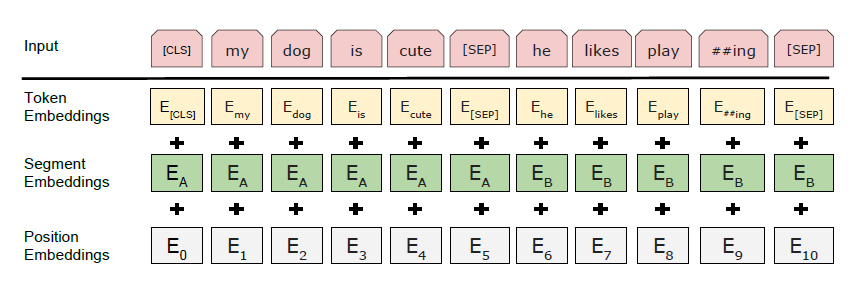
\includegraphics[width=\textwidth]{Figures/bert_inputrep.png}
    \caption{BERT input visualization for a sentence pair, A \& B. After \citet{devlin2018bert}.}
    \label{fig:berttokens}
\end{figure}

\subsubsection{Sentence-BERT}

A further development of BERT for representing sentences is Sentence-BERT. \citeauthor{reimers2019sentence} presented SBERT in \citeyear{reimers2019sentence}, where the main motivation was to be able to derive semantically meaningful sentence representations. The authors define semantic similarity as proximity in vector space, for instance measured by cosine similarity. SBERT uses a pre-trained BERT model and computes some pooling operation on the last layer. As seen in Figure \ref{fig:berttokens}, the length of the output sequence is equal to the input sequence. In order to get a fixed size representation of a sentence, the dimension is reduced to the same as the dimension of the words.

SBERT allows for three different pooling operations -- using the \textsc{[CLS]}-token, mean pooling or max-over-time pooling. The model is fine tuned using siamese and triplet networks. These are BERT networks with shared weights. Two sentences are fed into one network each and the similarity is compared between them. The authors explore different objective functions, one being mean squared error loss of the cosine similarity between two sentences. 


\section{Overfitting \& Hyperparameter Optimization}

This section concerns the problem of overfitting in a machine learning context. The contents in Sections \ref{sec:trainvaltest} through \ref{sec:crossval} mainly follow \citeauthor{Goodfellow-et-al-2016} but is covered thoroughly and in a similar fashion in most basic machine learning summaries. 

\subsection{Train, Validation, and Test Set}\label{sec:trainvaltest}

A popular definition of machine learning is quoted from \citeauthor{tommitchell1997}:
\begin{quote}
    \emph{``A computer program is said to learn from experience E with respect to some class of tasks T and performance measure P if its performance at tasks in T, as measured by P, improves with experience E.''}
\end{quote}

The main goal of machine learning is to be able to have some predictive power on previously unseen data. This is a difference between machine learning optimization and optimization in general. A model is said to \emph{generalize} well if it shows good performance on data it has not seen before. This is also how a model is typically used for some application -- we want to use the model to predict things of uncertainty, not things we already know. 

Suppose we have gathered a dataset $\mathcal{D}$ to train a model. In order to approximate how the model performs on unseen data, we can hide a partition of the dataset during training. Letting our initial dataset $\mathcal{D}$ be the set $\{\mathcal{D}_{train}, \mathcal{D}_{test}\}$, we optimize the model on the data $\mathcal{D}_{train}$ by minimizing some loss function $\mathcal{L}$ over the samples in $\mathcal{D}_{train}$. The generalization error of the trained model is then approximated by $\mathcal{L}(\mathcal{D}_{test})$.

The training of a machine learning model can be simply expressed as minimizing these two objectives:
\begin{enumerate}
    \item Minimize the training error.
    \item Minimize the difference between the training error and the test error. 
\end{enumerate}

If the training error is small while the difference between the training error and the test error is large, we say that the model has \emph{overfitted} to the training data. This usually means that the model has too high capacity and tries to represent too complex patterns. If the training error is large, but the difference between training error and test error is small, it indicates that the model is \emph{underfitted}. This implies that the model is not complex enough.  


A fundamental rule of machine learning is that the results on the test set can not influence the model structure in any way. The purpose of the test set is to estimate how well the model performs on new data. It is not a metric that is to be used for model optimization. Still, the objective is to optimize the model on unseen data. This is addressed by introducing a \emph{validation set}. 

Let the full dataset $\mathcal{D}$ be partitioned into three sets, $\{\mathcal{D}_{train}, \mathcal{D}_{validation}, \mathcal{D}_{test} \}$. The train set is then used to optimize the parameters of the model, while the validation set is not included in the training. The generalization error is approximated by the validation error. The validation error is by contrast to the test error however allowed to influence the model structure. This is typically done by adjusting the \emph{hyperparameters} of the model and introducing some \emph{regularization}, covered further in the following sections. 

\subsection{Hyperparameters}\label{sec:hyper}

A machine learning model is defined by its tuneable parameters and its hyperparameters. The tuneable parameters are normally just called parameters and are the trainable weights in a model. The hyperparameters are properties of the model that must be set before the training is started. Hyperparameters for a neural networks are typically the number of nodes in each layer, which activation function to use in the nodes, the depth of the network, what sort of optimization routine is used, the learning rate, etc. 

Many of these parameters can adjust the capacity of the network, i.e. how complex structures the network can model. If the model is too complex, it might be too sensitive to the training data and adapt to patterns in the training data which are not transferable to unseen data. If the model is not complex enough, it might fail to retrieve important patterns from the training data.

Other parameters rather adjust the speed and precision of training. The learning rate is such a parameter, deciding the size of the steps in the gradient descent-like optimization algorithm. A too big learning rate can imply that the optimization fails to  reach the sought minimum, a too small learning rate can imply that the optimization converges too slowly \citep{Goodfellow-et-al-2016}. 

\subsection{Regularization}\label{sec:regul}

Regularization is a way to prioritize more likely parameters over less likely parameters. It assumes we have some prior belief of which parameters that are more likely. The basic principle is the same as for Occam's razor -- if two solutions to a problem give equal results, choose the simplest one.

This concept is used to combat overfitting and to make the model focus on the most important patterns in the data. A model with high regularization is penalised for making complex decision rules, generally giving a higher training error. A simple way to introduce regularization is to add a \emph{weight decay} to the loss function. Given the weights $w$ in a neural network and some cost function $\mathcal{L}$, a new cost function $\mathcal{L}_R$ with weight decay can be constructed as in Eq. \ref{eq:weightdecay}.

\begin{align}
    \mathcal{L}_R (w) = \mathcal{L}(w) + \lambda w^T w
    \label{eq:weightdecay}
\end{align}

The parameter $\lambda$ is here a hyperparameter used to control the regularization strength. A higher $\lambda$ implies more regularization. 

\citeauthor{hinton2012improving} presented another regularization method used in the context of neural networks in \citeyear{hinton2012improving} --  \emph{dropout} regularization. This removes a node in the network with probability $p$ during every step in the optimization. It is arguably quite similar to training several different networks, since the network is constantly changing and removing nodes, altering its structure. Dropout can be seen as a cheap way of training and evaluating an ensemble of exponentially many neural networks. 

The nodes are only removed with probability $p$ during training. When the model is used for prediction, the weights of the nodes where dropout has been used is multiplied by $1 - p$. The argument for why this is reasonable is that seems to capture the correct expected value of the output from that node. Not a very theoretical argument, but it seems to work well \citep{hinton2012improving}. 


\subsection{Cross-Validation}\label{sec:crossval}

If the available dataset is small, it might be unrealistic to have the same statistical properties in the training, validation and test data. A small size also gives a large variance on both the validation and test set, making it difficult to select hyperparameters and estimate the performance on unseen data. A way to improve the accuracy of the estimate is to use \emph{k}-fold cross validation.  

\begin{figure}[H]
    \centering
    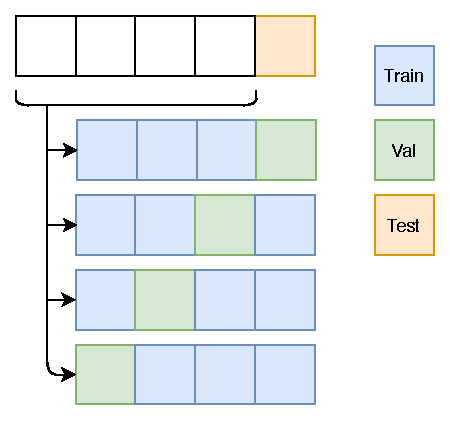
\includegraphics{Figures/figs-k-fold.pdf}
    \caption{Overview of how a dataset is used for $k$-fold cross validation with $k=4$. }
    \label{fig:kfold}
\end{figure}

Firstly, an independent test set is extracted from the dataset. The test set should have the same distribution of labels as the dataset. This is seen as the orange square in Figure \ref{fig:kfold}. The test set is typically 10-20 \% of the dataset, it does however depend on how large the dataset is.

The remaining samples in the dataset are then divided randomly into $k$ parts of equal size. A validation error with lower variance can then be calculated by taking the mean over all $k$ validation errors after fitting the model to the $k$ different training sets. This validation error can then be used to determine which set of hyperparameters gives the best performance. 

Finally, the performance of the model on unseen data is estimated on the test set with the hyperparameters found in the $k$-fold cross validation. If a more accurate test error is desired, an additional loop over $k$ test sets can be performed in a similar fashion as for the validation set. This is however not used for hyperparameter selection, only to get a better estimate of the generalization performance \citep{Goodfellow-et-al-2016}. 

\subsection{Grid Search \& Random Search}

Using the $k$-fold cross validation technique previously presented can be computationally expensive if a large set of hyperparameters are to be tested. Suppose we want to try the  number of hyperparameters in Table \ref{tab:hyper}. This gives 6750 combinations of parameters. Furthermore, using $k$-fold cross validation with $k=10$ would imply 67,500 fitted models in order to find the best set of hyperparameters. This might obviously be reasonable for smaller sets, but it rather quickly grows infeasible to do an exhaustive search over all possible combinations. 

\begin{table}[t]
    \centering
    \begin{tabular}{lr}
    \hline
        \textbf{Hyperparameter} & \textbf{\#} \\
        \hline \hline 
         Dropout rate & 3 \\
         Learning rate & 5 \\
         Hidden layers & 3 \\
         Nodes & 10 \\
         Optimizer & 5 \\
         Activation function & 3 \\
         Batch size & 5 \\
         \hline \hline 
         \textbf{Total \# combinations } & \textbf{6750}
    \end{tabular}
    \caption{}
    \label{tab:hyper}
\end{table}

A common and effective alternative is to use a random search. Only the possible distributions of the hyperparameters are defined, and a fixed number of combinations of these are evaluated. Random search finds good solutions quicker than grid search, as it reduces the validation error more for a given number of tested hyperparameters \citep{Goodfellow-et-al-2016}. 

\section{Performance Metrics}
The metrics used to evaluate the models are accuracy and F1-score. The F1-score is defined by the precision and recall, so these metrics are explained as well. For convenience a binary confusion matrix is displayed in Table~\ref{fig:confmat}. 

\begin{table}[ht]
\centering
\begin{tabular}{cccc}
     & & \multicolumn{2}{c}{Predictions} \\
     & & \multicolumn{1}{|c|}{0} & \multicolumn{1}{c|}{1}\\
      \cline{2-4}
     \multirow{2}{*}{Actual values} & 0 & \multicolumn{1}{|c|}{True Negatives (TN)} &  \multicolumn{1}{c|}{False Positives (FP)} \\
     %\cline{2-4}
      & 1 & \multicolumn{1}{|c|}{False Negatives (FN)} & \multicolumn{1}{c|}{True Positives (TP)} \\ 
\end{tabular}
\caption{Confusion matrix for binary classification.}
\label{fig:confmat}
\end{table}

\begin{description}
    \item[Accuracy:] The most intuitive measure of performance, simply the ratio of correct classifications to the total number of classifications. If the labels of a data set are symmetric, this is a good measure of performance. However, if 90 \%  of the samples are of label $a$ and 10\% of label $b$, a model which constantly predicts label $a$ gets an accuracy of 90\%. It doesn't reveal any information about which data is classified incorrectly. 
    \item[Precision:] The number of correctly classified samples in one class divided by the total number of predictions of that class. The precision $P$ for class 0 in Table~\ref{fig:confmat} is calculated as $\displaystyle{P = \frac{TN}{TN + FN}}$. 
    \item[Recall:] The number of correctly classified samples in one class divided by the total number of samples in that class. In other words, a measure of how many percent of a class that was found. In relation to Table~\ref{fig:confmat} it is calculated as $\displaystyle{R = \frac{TN}{TN + FP}}$. Recall is also referred to as \textit{sensitivity} in statistical literature. 
    \item[F1-score:] A measure which combines precision and recall as the harmonic mean of the two. Calculated as $\displaystyle{F1 = 2 \frac{R \cdot P}{R + P}}$. An F1-score of 1 implies perfect recall and precision.
\end{description}

The precision, recall and F1-score are metrics which are calculated for every class in a classification problem. In order to get a single metric for a set of samples, these can be weighted by the number of true labels of each class. Hence for a binary classification problem, $F1_w = F1_0 \cdot w_0 + F1_1 \cdot w_1$, where $w_i$ is the ratio of labels in class $i$ in the training set \citep{Ting2017}. A more interesting metric for a skewed data set is the macro F1-score, which averages the F1-score for each label regardless of the ratio of labels. Consider a dataset with 99\% of label \emph{A} and 1\% label \emph{B}. If a classifier predicts \emph{A} for all targets, the weighted F1-score would be $\displaystyle{F1_w = 1 \cdot \frac{99}{100} + 0 \cdot \frac{1}{100} = \frac{99}{100}}$. The macro F1-score would simply take the average over both F1-scores, i.e. $F1_m = 0.5$. This is arguably a more reasonable measure for a skewed set of labels. 

